
%|  Name  | TODO | ONGOING | DONE |
%|--------|------|---------|------|
%| Dana   | x    |         |      |
%| Gerd   |      |         |  x   |
%| Glenn  |      |         |  x   |
%| Jordan | x    |         |      |
%| Luke   | x    |         |      |
%| Matt   |      |         |  x   |
%| Neil   | x    |         |      |
%| Scot   | x    |         |      |

A somewhat twisted reading of `Hierarchical Data Format' might create the idea that there might be something hierarchical about the file format. There indeed are a few discernible layers in the file format specification~\cite{ffmt}, and we used the TCP/IP protocol metaphor (see Figure~\ref{fig:tcpip-protocols}) to explain how the native VOL frames user metadata and data into portable self-describing packages, but this would be a rather uninteresting hierarchy, and none that would help users. What's hierarchical about HDF5 is how the object namespace is realized through groups and links, which differs fundamentally from hierarchies that can be mimicked in key-value representations. Not only is the file-system-in-a-file metaphor apt, but an HDF5 file is also a \textit{web-in-a-file}.

\subsection{Groups}

\paragraph{Overview} Groups are a key aspect of an HDF5 file's hierarchical structure. A minimal example of group creation is shown in Listing~\ref{lst:group-life-cycle}.

It is often said that named HDF5 objects (datasets, groups, and committed datatypes) reside in groups. To be more precise, groups contain link objects that point to named HDF5 objects. When a named object is created, a link that points to it is also created. It is this link that is written to the group's object header in storage. This is why \func{H5Dcreate}, \func{H5Tcommit}, and \func{H5Gcreate} all take a link creation property list as an argument.

Figure~\ref{fig:tour-4-uml-group-create} shows the library's internal process to create a new group through the native VOL. The application calls the API function \func{H5Gcreate}, and because groups are (generally) named objects, \func{H5G__create_named} is invoked. After creating a new group in an HDF5 file, \func{H5L_link_object} links it into the HDF5 file hierarchy. This linking process involves creating a link using \func{H5L__create_real} that points to the newly created group. The link is then stored in the parent group of the new object, which, in this case, is the root group.


\begin{listing}
\centering
\caption{Group life cycle.}
\label{lst:group-life-cycle}
\begin{minted}[linenos]{C}
#include "common.h"
int main() {
  hid_t file_id = H5Fcreate("groups.1.h5", H5F_ACC_TRUNC, H5P_DEFAULTx2);
  hid_t group_id = H5Gcreate(file_id, "grp1", H5P_DEFAULTx3);
  H5Gclose(group_id);
  H5Fclose(file_id);
  return 0;
}
\end{minted}
\end{listing}

\begin{comment}
https://www.plantuml.com/plantuml/
@startuml
participant H5G
participant H5L

rnote over H5G: H5Gcreate()
rnote over H5G: (...)
H5G -> H5L: H5G__create_named()
rnote over H5L: H5L_link_object()
rnote over H5L: H5L__create_real()
H5L -> H5G: Return new group info

rnote over H5G: Finish group creation
@enduml
\end{comment}

\begin{figure}
    \centering
    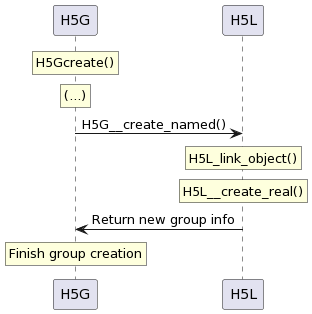
\includegraphics[width=0.40\textwidth]{images/tour_4_group_create.png}
    \caption{The library internally creates a link to a new named group}
    \label{fig:tour-4-uml-group-create}
\end{figure}

\paragraph{The Root Group} Every HDF5 file is created with a single named object - the root group. The root group has the fixed name \texttt{/}, and acts as the root of a file's hierarchy. It is the only group that does not need to reside within a group itself. The root group is closely associated with the file itself - when API functions operate on HDF5 files as objects, they often act on the root group internally.

\begin{comment}
\paragraph{Intermediate Group Creation} Figure~\ref{fig:group-intermediate-creation} shows an example of creating multiple nested groups with a single API call.

\begin{listing}
\centering
\caption{Intermediate Group Creation}
\label{lst:group-intermediate-creation}
\begin{minted}[linenos]{C}
#include "common.h"
int main() {
    hid_t file_id = H5Fcreate("group.h5", H5F_ACC_TRUNC, H5P_DEFAULTx2);
    hid_t lcpl = H5Pcreate(H5P_LINK_CREATE);
    H5Pset_create_intermediate_group(lcpl, 1);
    H5Gclose(H5Gcreate(file_id, "group1/group2/group3", lcpl,
        H5P_DEFAULTx2));
    H5Pclose(lcpl);
    H5Fclose(file_id);
    return 0;
}
\end{minted}
\end{listing}
\end{comment}

\subsection{Links}

\paragraph{Overview} The structure of an HDF5 file is a rooted, directed graph. Named objects form the nodes of this graph, and links are the edges between them. Links point from a group to a target object, and may be 'traversed' from their parent group to access the target object. Links are indexed within a group, allowing them to be iterated through recursively with \func{H5Lvisit} or non-recursively with \func{H5Literate}.

When a named object is created in a particular group, a hard link pointing to it is created and placed in that group. Hard links store the physical address of the object in the file. Other types of links, which use a name or other symbol to point to an object rather than its physical address, are called 'symbolic links'.

\paragraph{Hard Links and Objects} Each time a hard link to an object is created or destroyed, the target object's internal count of how many links point to it, the field \texttt{nlink} in the \texttt{H5O\_t} struct, is updated accordingly.

When an object has no links pointing to it, it becomes inaccessible in the file and the space it occupies is marked as 'free' by the file's free space manager. Unless persistent free space management is enabled on the file, this free space tracking information will be lost when the file is closed, and the memory will not be reclaimed until a tool such as \texttt{h5repack} is used.

In the context of HDF5, "reference count" refers to in-memory objects tracking how many other in-memory objects reference them, and the term has no relation to the number of links to an object in the file hierarchy.

\begin{comment}
https://www.plantuml.com/plantuml
@startuml
participant H5L
participant H5G
participant H5O

rnote over H5L: H5Lcreate_(hard/soft/external/ud)

alt Hard Link
rnote over H5L: H5L__create_hard
else Soft Link
rnote over H5L: H5L__create_soft
else External/User-defined Link
rnote over H5L: H5L__create_ud
end

H5L -> H5G: H5L__create_real
H5G -> H5L: H5G_traverse
H5L -> H5G: H5L__link_cb
H5G -> H5O: H5G_obj_insert

opt Hard Link
rnote over H5O: H5O_link
end
@enduml
\end{comment}

\begin{figure}
    \centering
    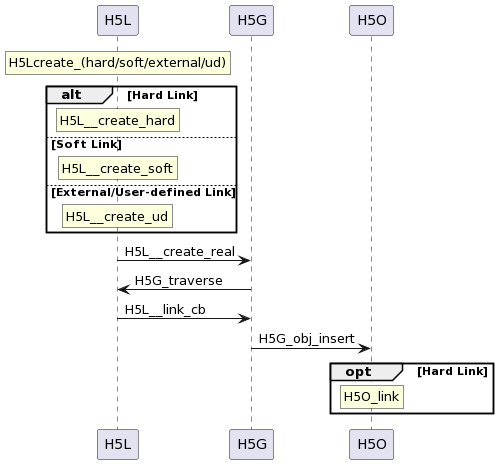
\includegraphics[width=0.6\textwidth]{images/tour_4_uml_link_create.png}
    \caption{Link creation sequence diagram}
    \label{fig:tour-4-uml-link-create}
\end{figure}

\paragraph{Link Creation} Figure~\ref{fig:tour-4-uml-link-create} illustrates the library's process for link creation. After link-type-specific setup is done by \func{H5L__create_[hard/soft/external/ud]}, the link object is created by \func{H5L__create_real}.

The API's link creation functions require both a location identifier and a name for the link that will be created. This link name may be a relative path from the object specified by the location identifier, or an absolute path from the root of the file. If the provided link name is a path with intermediate elements, then \func{H5G_traverse} is used to traverse the path and create the link object at the correct place in the file hierarchy. Once the final destination for the new link is reached, the link is inserted into the group containing it with \func{H5G_obj_insert}. If it is a hard link, \func{H5O_link} increments the target object's \texttt{nlink} count.

\paragraph{Soft Links} Soft links are a type of symbolic link that point to a path in the file hierarchy rather than an address in the file. When a soft link is created, no checks are performed to ensure that an object exists at the target path. A link that does not point to an existing object is called a dangling link. Allowing soft links to dangle means that changing, removing or entirely replacing an object that resides at a location pointed to by soft links can be done without additional work on the part of the library or the application.

\begin{listing}
\centering
\caption{Soft link example}
\label{lst:soft-link-example}
\begin{minted}[linenos]{C}

#include "common.h"
int main() {
  hid_t file_id = H5Fcreate("groups.1.h5", H5F_ACC_TRUNC, H5P_DEFAULTx2);
  hid_t group_id = H5Gcreate(file_id, "grp1", H5P_DEFAULT, H5P_DEFAULTx2);
  hid_t space_id = H5Screate(H5S_SCALAR);

  H5Lcreate_soft("/grp1/data", group_id, "link_to_data", H5P_DEFAULTx2);
  hid_t dset_id = H5Dcreate(group_id, "data", H5T_NATIVE_INT, space_id,
    H5P_DEFAULTx3);
  H5Dclose(dset_id);

  dset_id = H5Dopen(group_id, "link_to_data", H5P_DEFAULT);
  H5Dclose(dset_id);
  H5Sclose(space_id);
  H5Gclose(group_id);
  H5Fclose(file_id);
  return 0;
}

\end{minted}
\end{listing}

\begin{comment}
https://www.plantuml.com/plantuml/
@startuml
participant H5D
participant H5G

rnote over H5D: H5Dopen
H5D -> H5G: H5D__open_name

rnote over H5G: H5G_loc_find
rnote over H5G: H5G_traverse
rnote over H5G: H5G_traverse_real
group Non-Hard Link
rnote over H5G: H5G__traverse_(slink/ud)
end
rnote over H5G: H5G__loc_find_cb

H5G -> H5D: Return dataset location info
@enduml
\end{comment}

\begin{figure}
    \centering
    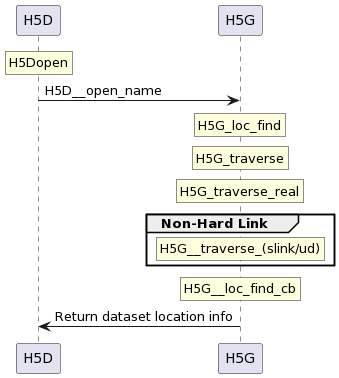
\includegraphics[width=0.40\textwidth]{images/tour_4_uml_link_access.png}
    \caption{Sequence diagram of opening a dataset through a link}
    \label{fig:tour-4-uml-link-access}
\end{figure}

\paragraph{Accessing Objects Through Links} Figure~\ref{fig:tour-4-uml-link-access} shows the process the library uses to access an object through a link.

After the VOL layer is passed through and the native \func{H5D__open_name} is invoked, \func{H5G_loc_find} is called in order to retrieve the two components of the location of the dataset - the path to it in the file hierarchy and its address in physical storage. This function invokes \func{H5G_traverse} to traverse the path to the link, as well as the path the link contains if it is a soft or external link. \func{H5G_loc_find} also provides the traversal function with the \func{H5G__loc_find_cb} callback to be used upon locating the target object. This callback copies the target object's group location information. After the location information is retrieved, the rest of the type-specific object opening work is performed.

\begin{listing}
\centering
\caption{Creating and using a user-defined link class}
\label{lst:ud-link-example}
\begin{minted}[linenos]{C}
#include <string.h>
#include "common.h"
hid_t UD_soft_traverse(const char *link_name, hid_t cur_group,
                       const void *udata, size_t udata_size,
                       hid_t lapl_id, hid_t dxpl_id) {
  const char *target_obj_name = (const char *)udata;
  hid_t ret_value = H5Oopen(cur_group, target_obj_name, lapl_id);
  return ret_value;
}

const H5L_class_t UD_soft_class[1] = {{
    H5L_LINK_CLASS_T_VERS,             /* Version number for this struct */
    (H5L_type_t)H5L_TYPE_EXTERNAL + 1, /* Link class id number.          */
    "UD_soft_link",                    /* Link class name for debugging  */
    NULL,             NULL, NULL,      /* Link class op callbacks        */
    UD_soft_traverse, NULL, NULL
}};

int main() {
  hid_t file_id = H5Fcreate("ud_link.h5", H5F_ACC_TRUNC, H5P_DEFAULTx2);
  H5Lregister(UD_soft_class);
  /* Pass the path to the root group as udata */
  H5Lcreate_ud(file_id, "ud_link", (H5L_type_t)H5L_TYPE_EXTERNAL + 1, "/",
               strlen("/") + 1, H5P_DEFAULTx2);

  hid_t group_id = H5Gopen2(file_id, "ud_link", H5P_DEFAULT);
  H5Gclose(group_id);
  H5Fclose(file_id);
  return 0;
}

\end{minted}
\end{listing}

\paragraph{User-defined Links} As part of the library's effort to be as extensible as possible, users may define and register their own link types. \func{H5Lregister} can be used to register a new link class, after which an instance of the new link class may be created with \func{H5Lcreate_ud}.

Listing ~\ref{lst:ud-link-example} shows a minimal example of a user-defined link class, which mimics the behavior of soft links. The only callback that must be defined is the traversal callback, which handles obtaining an object handle from a link pointing to that object. The other callbacks - create, move, copy, delete, and query - all have some baseline functionality implemented by the library, with the user's callback being invoked after the internal work is completed. For example, for a user-defined link class with no provided query callback, \func{H5Lget_info} will still return the character set of the link's name, its creation order in its parent group, whether its creation order is valid, and the link's type. However, the returned size of the link will default to zero unless the query operation is implemented.

\subsection{Link Storage}

\paragraph{Overview}  Similar to attributes, there are two ways that links may be stored in a file: compact and dense. Compactly stored links are kept in the object header for the group containing them, along with other metadata for that group object. Densely stored links are kept in a fractal heap. The address of the dense link fractal heap is stored in the Link Info message in the group's header, with the heap IDs to access specific dense links stored in a name index B-tree.

Older versions of the file format stored all links in a symbol table. A symbol table will still be used for link storage if the 'low' library compatibility version on a file is set lower than 1.8. By default, a new file has its 'low' compatibility version set to \texttt{H5F\_LIBVER\_EARLIEST}, which will disable use of the fractal heap for dense link storage.

Links are stored compactly if two criteria are met: the link message is under 64 KiB in size, and the number of links is below the maximum number of compact links on the group. The maximum number of compact links on a group may be set at creation time via \func{H5Pset_link_phase_change}. If either of these criteria are not met, the new link will be put into dense storage, and any existing compact links will be converted to dense storage. If the number of links later drops below the minimum number of compact links set by \func{H5Pset_link_phase_change}, then any links below 64 KiB will be converted to compact storage.

\begin{comment}
https://www.plantuml.com/plantuml/
@startuml
participant H5D
participant H5G
participant H5HF
participant H5B2

rnote over H5D: H5Dcreate
H5D -> H5G: (...)
rnote right: H5G_obj_insert

opt Fractal heap does not yet exist
rnote over H5G: H5G__dense_create
H5G -> H5HF: Create fractal heap in the file
rnote right: H5HF_create
H5G -> H5B2: Create name index B-tree
rnote right: H5B2_create

opt If creation order is tracked
H5G -> H5B2: Create creation order B-tree
rnote right: H5B2_create
end
end

rnote over H5G: H5G__dense_insert
H5G -> H5HF: Insert link into fractal heap
rnote right: H5HF_insert
H5G -> H5B2: Insert link into name B-tree
rnote right: H5B2_insert
opt If creation order is tracked
H5G -> H5B2: Insert record into creation order B-tree
rnote right: H5B2_insert
end

@enduml
\end{comment}

\begin{figure}
    \centering
    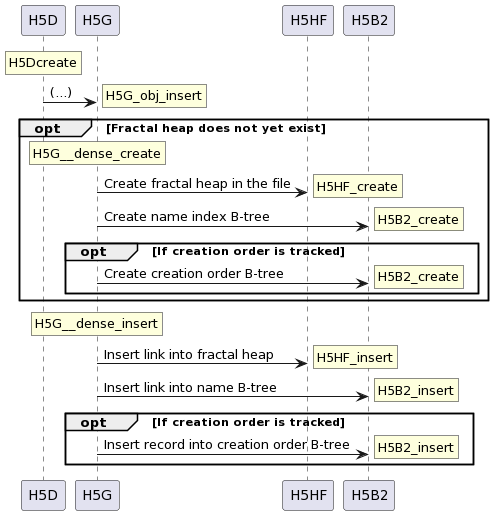
\includegraphics[width=0.6\textwidth]{images/tour_4_uml_link_storage_dense.png}
    \caption{Link insertion into dense storage during dataset creation}
    \label{fig:tour-4-uml-link-storage-dense}
\end{figure}


\begin{comment}
https://www.plantuml.com/plantuml/
@startuml
participant H5D
participant H5G

rnote over H5D: H5Dcreate
H5D -> H5G: (...)
rnote right: H5G_obj_insert

H5G -> H5O: H5G__compact_insert
rnote right: H5O_msg_create

hnote over H5O #FFAAAA: Object header is pinned
rnote over H5O: H5O_msg_append_oh
rnote over H5O: H5O__msg_alloc
rnote over H5O: H5O__copy_mesg

hnote over H5O #FFAAAA: Object header is unpinned
@enduml
\end{comment}

\begin{figure}
    \centering
    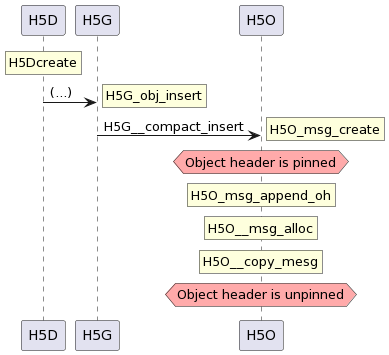
\includegraphics[width=0.5\textwidth]{images/tour_4_uml_link_storage_compact.png}
    \caption{Link insertion into compact storage during dataset creation}
    \label{fig:tour-4-uml-link-storage-compact}
\end{figure}

\paragraph{Inserting Links into Storage} An example of link insertion into dense storage is illustrated in Figure~\ref{fig:tour-4-uml-link-storage-dense}. If the file does not yet have the structures needed to store dense links, they are created in \func{H5G__dense_create}. This involves creating a fractal heap for dense links via \func{H5HF_create}, creating a B-tree to hold the names of dense links via \func{H5B2_create}, and, if creation order is tracked on the parent group, creating another B-tree to track creation order. Once the the structures for dense storage are confirmed to exist, insertion into dense storage is handled by \func{H5G_dense_insert}. The insertion into the fractal heap itself is done by \func{H5HF_insert}. The name-index B-tree stores information about the link that may later be accessed by the hash of the link name, and the creation-order B-tree stores the same information with the link creation index as the key.

\begin{comment}
https://www.plantuml.com/plantuml
@startuml
participant H5D
participant H5G
participant H5O

rnote over H5D: H5Dopen
H5D -> H5G: (...)
rnote right: H5G_traverse

group Link is compact

H5G -> H5O: H5G__compact_lookup
rnote over H5O: H5O_msg_iterate
H5O -> H5G:
rnote over H5G: H5G__compact_lookup_cb
H5G -> H5O: If link found by name
end
rnote over H5O: H5O_msg_copy
H5O -> H5G: Return link info
H5G -> H5D: Return dataset handle
@enduml
\end{comment}

\begin{figure}
\centering
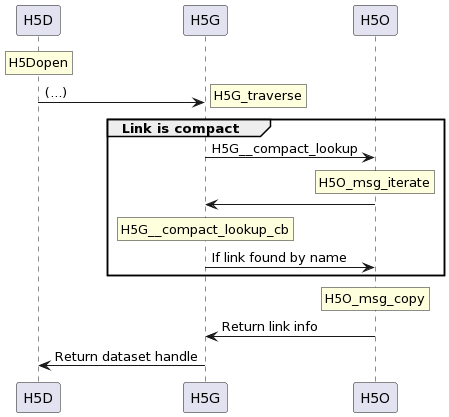
\includegraphics[width=0.55\textwidth]{images/tour_4_uml_link_access_compact.png}
\caption{How the library accesses a compact link}
\label{fig:tour-4-uml-link-access-compact}
\end{figure}

\begin{comment}
https://www.plantuml.com/plantuml
@startuml
participant H5D
participant H5G
participant H5O
participant H5HF
participant H5B2

rnote over H5D: H5Dopen
H5D -> H5G: (...)
rnote right: H5G_traverse

group Link to dataset is dense
rnote over H5G: H5G__dense_lookup
H5G -> H5HF: Open fractal heap of file
rnote right: H5HF_open

H5G -> H5B2: Open name index B-tree
rnote right: H5B2_open
H5G -> H5B2: Search for link name in B-tree
rnote right:H5B2_find

H5B2 -> H5G: If dense link is found by name
rnote over H5G: H5G__dense_lookup_cb
H5G -> H5O: Copy link message from header
end

rnote over H5O: H5O_msg_copy
H5O -> H5G: Return link info
H5G -> H5D: Return dataset handle
@enduml
\end{comment}

\begin{figure}
\centering
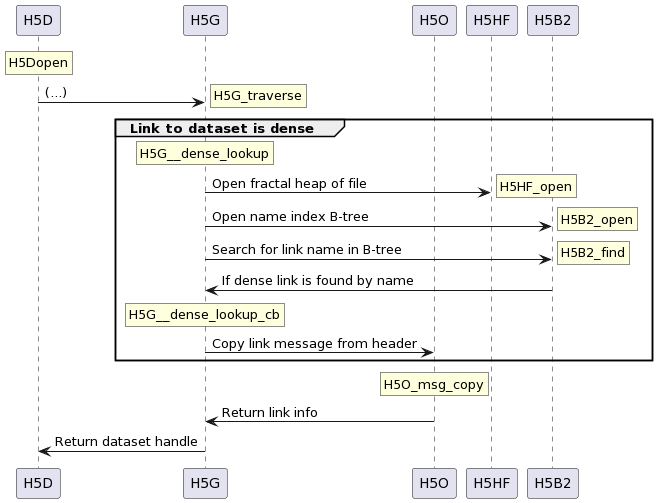
\includegraphics[width=0.70\textwidth]{images/tour_4_uml_link_access_dense.png}
\caption{How the library accesses a dense link}
\label{fig:tour-4-uml-link-access-dense}
\end{figure}

The process for compact link insertion into the object header is illustrated in Figure~\ref{fig:tour-4-uml-link-storage-compact}. Compact links are inserted by \func{H5G__compact_insert}. \func{H5G_msg_create} sets up the message to be inserted. Before the message is appended onto the object header, the object header is "pinned" with \func{H5O_pin}. Pinning the object header prevents it from being written from cache to storage in the middle of operations that modify the header. \func{H5O_msg_append_oh} appends the newly created message to the object header. This is done in two parts: first \func{H5O__msg_alloc} creates space in the object header, then \func{H5O__copy_mesg} populates the allocated memory with link message information. Lastly, the object header is unpinned by \texttt{H5O\_unpin()}, allowing it to be flushed from cache again.

\paragraph{Accessing Links in Storage} Figures~\ref{fig:tour-4-uml-link-access-compact} and \ref{fig:tour-4-uml-link-access-dense} illustrate the library's process for accessing objects through links in compact and dense storage, respectively.

\func{H5G_traverse} is used regardless of storage type to locate the link through the provided path in the file hierarchy. Once the correct location in the hierarchy is reached, the process branches based on how the link is stored.

If the link is compact, \func{H5G__compact_lookup} searches the object header for a message describing a link of the correct name. \func{H5O_msg_iterate} iterates through each message and uses \func{H5G_compact_lookup_cb} to copy the link information if a match is found.

If the link is dense, \func{H5G__dense_lookup} does the name lookup. The dense link fractal heap and the name index B-tree are both opened. \func{H5B2_find} searches name index B-tree for the dense link. If a match is found, the provided callback \func{H5G__dense_lookup_cb} copies the link information.

In both cases, once the link is found by name, its information is copied with \func{H5O_msg_copy} and returned to \func{H5G_traverse}. The link traversal callback for the link's type is used to access information about the object through the link, and a handle to the object is returned by the top-level open function.

\subsection{Summary} Implementing group membership via links introduces a layer of indirection to the file hierarchy which is extremely powerful. Based on the use case of the application, objects can be accessed based on storage location, path within the file hierarchy, path in the filesystem via external links, or something else entirely with user-defined link classes. Since scalability with extremely large amounts of data is a core goal of the HDF5 library, maximizing the user's ability to manipulate the file hierarchy without affecting the underlying arrangement of data is critical.

Scalability with large numbers of links in a group was another important design goal, realized in the architecture by dense link storage. The tradeoff between compact storage being better for small numbers of links and dense storage being better for large numbers of links is automatically handled during operation by the maximum compact/minimum dense thresholds, and may also be custom-fit to a use case by the user through manipulating property lists.
